\documentclass{article}

\usepackage{amsmath,amssymb}
\usepackage{tikz}
\usepackage{pgfplots}
\usepackage{xcolor}
\usepackage[left=2.1cm,right=3.1cm,bottom=3cm,footskip=0.75cm,headsep=0.5cm]{geometry}
\usepackage{enumerate}
\usepackage{enumitem}
\usepackage{marvosym}
\usepackage{tabularx}

\usepackage[utf8]{inputenc}

\renewcommand*{\arraystretch}{1.4}

\newcolumntype{L}[1]{>{\raggedright\arraybackslash}p{#1}}
\newcolumntype{R}[1]{>{\raggedleft\arraybackslash}p{#1}}
\newcolumntype{C}[1]{>{\centering\let\newline\\\arraybackslash\hspace{0pt}}m{#1}}

\title{\textbf{Rechtfertigung der Staatstätigkeit, Hausaufgabe 2}}
\author{\textsc{Henry Haustein}}
\date{}

\begin{document}
	\maketitle
	
	\section*{Aufgabe 1}
	\begin{enumerate}[label=(\alph*)]
		\item Zuerst müssen wir die Funktion $x(p)$ in die Form $p(x)$ bringen: 
		\begin{align}
			200-20p &= x \notag \\
			200-x &= 20p \notag \\
			10-\frac{x}{20} &= p \notag
		\end{align}
		Die optimale Menge ist da, wo $GZB=GK$ ist:
		\begin{align}
			GK &= GZB \notag \\
			2 &= 10-\frac{x}{20} \notag \\
			x^{opt} &= 160 \notag
		\end{align}
		\item Der Monopolist maximiert seinen Gewinn, also $\Pi = x\cdot p-2x\to\max$:
		\begin{align}
			\Pi &= x\left(10-\frac{x}{20}\right)-2x \notag \\
			\frac{\partial \Pi}{\partial x} &= 10-\frac{x}{10}-2 = 0 \notag \\
			8 &= \frac{x}{10} \notag \\
			x^{mon} &= 80 \Rightarrow p^{mon}=6 \notag
		\end{align}
		\item Diagramm
		\begin{center}
			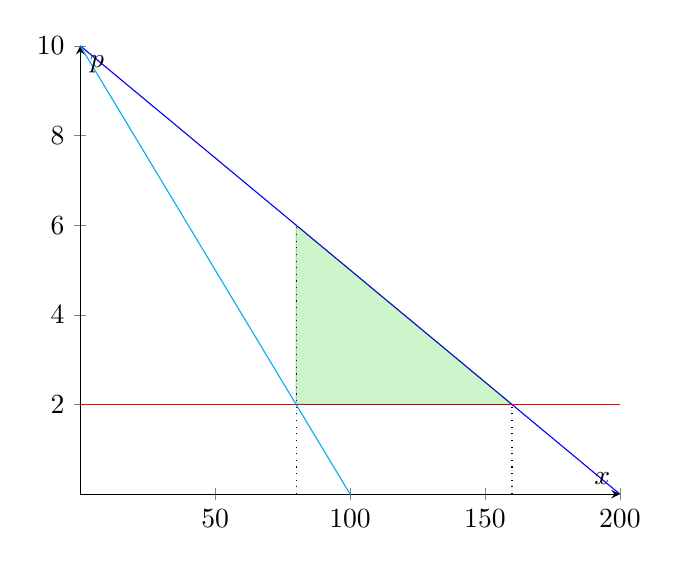
\begin{tikzpicture}
				\begin{axis}[
					xmin=0, xmax=200, xlabel=$x$,
					ymin=0, ymax=10, ylabel=$p$,
					samples=400,
					axis x line=middle,
					axis y line=middle,
					domain=0:200,
					]
					\addplot[mark=none,smooth,blue] {10-x/20};
					\addplot[mark=none,smooth,red] {2};
					\addplot[mark=none,smooth,cyan] {10-x/10};
					
					\draw[dotted] (axis cs: 80,0) -- (axis cs: 80,6);
					\draw[dotted] (axis cs: 160,0) -- (axis cs: 160,2);
					
					\draw[fill=green!80!black,opacity=0.2] (axis cs: 80,2) -- (axis cs: 80,6) -- (axis cs: 160,2) -- (axis cs: 80,2);
				\end{axis}
			\end{tikzpicture} \\
			\textcolor{blue}{GZB}, \textcolor{red}{GK}, \textcolor{cyan}{GE = $10-\frac{x}{10}$}, \textcolor{green!80!black}{Wohlfahrtsverlust}
		\end{center}
		\item Der Wohlfahrtsverlust entsteht durch die Verknappung des Outputs. Es gibt jenseits von $x^{mon}$ noch Kunden, die mehr bezahlen würden als die Produktion einer weiteren Einheit kostet.
		\item Der Wohlfahrtsverlust ist
		\begin{align}
			WFV &= \frac{1}{2}(x^{opt}-x^{mon})(p^{mon}-p^{opt}) \notag \\
			&= \frac{1}{2}(160-80)(6-2) \notag \\
			&= 160 \notag
		\end{align}
	\end{enumerate}
	
	\section*{Aufgabe 2}
	\begin{enumerate}[label=(\alph*)]
		\item Der Monopolist setzt $GE=GK$. Die Grenzkosten sind gegeben, kümmern wir uns um den Grenzerlös:
		\begin{align}
			E &= p\cdot x \notag \\
			&= (a-bx)\cdot x \notag \\
			&= ax - bx^2 \notag \\
			GE &= a - 2bx \notag
		\end{align}
		Setzen wir ein
		\begin{align}
			GE &= GK \notag \\
			a-2bx &= cx+d \notag \\
			a-d &= cx+2bx \notag \\
			x_M &= \frac{a-d}{c+2b} \notag
		\end{align}
		Aus sozialer Sicht wäre $GK=GZB$ wünschenswert, also
		\begin{align}
			cx+d &= a-bx \notag \\
			cx+bx &= a-d \notag \\
			x_{opt} &= \frac{a-d}{c+b} \notag
		\end{align}
		\item Eine Subvention senkt die Grenzkosten des Monopolisten. Man muss also solange subventionieren, bis $GE=GK-s \Rightarrow x_{opt}=\frac{a-d}{b+c}$ ergibt.
		\begin{align}
			a-2bx_S &= cx_S+d-s \notag \\
			a-d+s &= cx_S + 2bx_S \notag \\
			x_S &= \frac{a-d+s}{c+2b} \notag \\
			&\overset{!}{=} \frac{a-d}{b+c} \notag \\
			(c+2b)(a-d) &= (a-d+s)(b+c) \notag \\
			a-d+s &= \frac{(c+2b)(a-d)}{b+c} \notag \\
			s &= \frac{(c+2b)(a-d)}{b+c}-a+d \notag \\
			&= \frac{b(a-d)}{b+c} \notag
		\end{align}
		\item Subventionsbedarf: $S = s\cdot x = \frac{(a-d)^2b}{(b+c)^2}$
		\begin{center}
			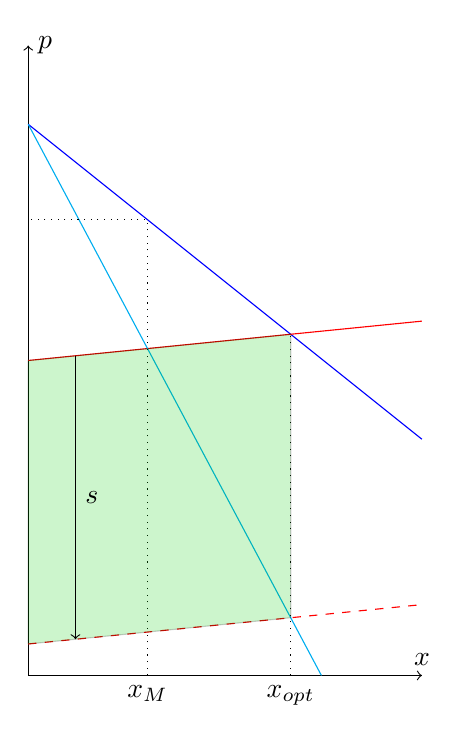
\begin{tikzpicture}
				\draw[->] (0,-3) -- (5,-3) node[above] {$x$};
				\draw[->] (0,-3) -- (0,5) node[right] {$p$};
				
				\draw[blue] (0,4) -- (5,0);
				\draw[red] (0,1) -- (5,1.5);
				\draw[dashed,red] (0,-2.6) -- (5,-2.1);
				\draw[cyan] (0,4) -- (175/47,-3);
				
				\draw[dotted] (50/33,-3) node[below] {$x_M$} to (50/33,92/33) -- (0,92/33);
				\draw[dotted] (10/3,-3) node[below] {$x_{opt}$} to (10/3,4/3);
				
				\draw[fill=green!80!black,opacity=0.2] (0,-2.6) -- (10/3,-34/15) -- (10/3,4/3) -- (0,1) -- (0,-2.6);
				
				\draw[->] (0.6,1.06) to node[midway,right] {$s$} (0.6,-2.54);		
			\end{tikzpicture} \\
			\textcolor{blue}{GZB}, \textcolor{red}{GK/um $s$ reduzierte Grenzkosten}, \textcolor{cyan}{GE}, \textcolor{green!80!black}{Subventionsbedarf}
		\end{center}
		\item Diese Subvention ist teuer und "schwierig zu verkaufen": Man belohnt einen Monopolisten dafür, dass er ein Monopol hat, statt ihn zu zerschlagen. Etwas billiger wird es, wenn man nur die Einheiten zwischen $x_M$ und $x_{opt}$ subventioniert.
		\begin{center}
			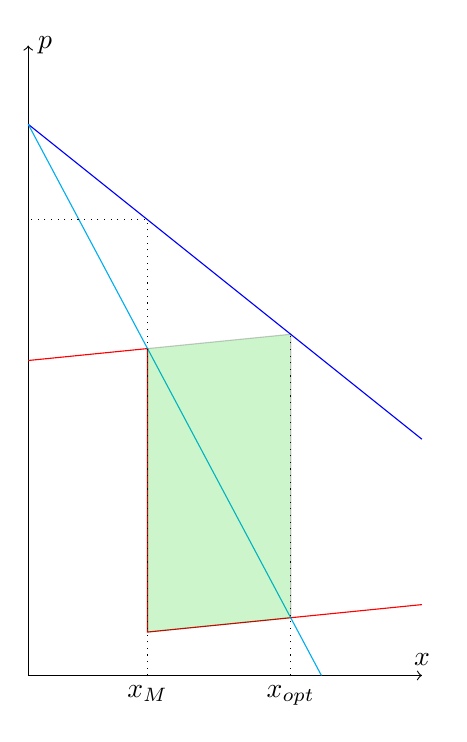
\begin{tikzpicture}
				\draw[->] (0,-3) -- (5,-3) node[above] {$x$};
				\draw[->] (0,-3) -- (0,5) node[right] {$p$};
				
				\draw[blue] (0,4) -- (5,0);
				\draw[red] (0,1) -- (50/33,38/33) -- (50/33,-404/165) -- (5,-2.1);
				\draw[cyan] (0,4) -- (175/47,-3);
				
				\draw[dotted] (50/33,-3) node[below] {$x_M$} to (50/33,92/33) -- (0,92/33);
				\draw[dotted] (10/3,-3) node[below] {$x_{opt}$} to (10/3,4/3);
				
				\draw[fill=green!80!black,opacity=0.2] (50/33,-404/165) -- (10/3,-34/15) -- (10/3,4/3) -- (50/33,38/33) -- (50/33,-404/165);
			\end{tikzpicture} \\
			\textcolor{blue}{GZB}, \textcolor{red}{um $s$ reduzierte Grenzkosten}, \textcolor{cyan}{GE}, \textcolor{green!80!black}{Subventionsbedarf}
		\end{center}
	\end{enumerate}

	\section*{Zusatzaufgabe 1}
	\begin{enumerate}[label=(\alph*)]
		\item Zuerst müssen wir die Funktion $x(p)$ in die Form $p(x)$ bringen:
		\begin{align}
			x &= 4-\frac{p}{3} \notag \\
			\frac{p}{3} &= 4-x\notag \\
			p &= 12-3x \notag
		\end{align}
		Die optimale Menge ist bei $GZB=GK$:
		\begin{align}
			GK &= GZB \notag \\
			6 &= 12-3x \notag \\
			x^{opt} &= 2 \notag
		\end{align}
		\item Der Monopolist betrachtet $GE=GK$, wobei $GE=E'=[12x-3x^2]'=12-6x$:
		\begin{align}
			GK &= GE \notag \\
			6 &= 12-6x \notag \\
			x^{mon} &= 1 \Rightarrow p^{mon}=9 \notag
		\end{align}
		\item Der Wohlfahrtsverlust ist
		\begin{align}
			WFV &= \frac{1}{2}(x^{opt}-x^{mon})(p^{mon}-p^{opt}) \notag \\
			&= \frac{1}{2}(2-1)(9-6) \notag \\
			&= \frac{3}{2} \notag
		\end{align}
		\item Der Gewinn des Monopolisten ist
		\begin{align}
			\Pi &= x\cdot GZB - K(x) + s\cdot x \notag \\
			&= 12x-3x^2 - 6x + sx \to\max \notag
			\frac{\partial \Pi}{\partial x} &= 12-6x-6+x = 0 \notag \\
			6x &= 6+s \notag \\
			x^{mon} &= 1+\frac{s}{6} \overset{!}{=} x^{opt} \notag
			1+\frac{s}{6} &= 2 \notag \\
			s &= 6 \notag
		\end{align}
		Der Subventionsbedarf ist dann $S=6\cdot 2=12$.
	\end{enumerate}

	\section*{Aufgabe 3}
	\begin{enumerate}[label=(\alph*)]
		\item Der Monopolist maximiert seinen Gewinn, dieser ist gegeben durch
		\begin{align}
			\Pi &= (10-F(N,K))\cdot F(N,K) - wN - rK \notag \\
			&= 10\sqrt{K}\sqrt{K} - \sqrt{K}\sqrt{N}\cdot\sqrt{K}\sqrt{N} - wN -  rK \notag
		\end{align}
		Ableiten nach $K$ und $N$ liefert die optimalen Faktoreinsatzmengen:
		\begin{align}
			\frac{\partial\Pi}{\partial K} &= \frac{10\sqrt{N}}{2\sqrt{K}} - N - r = 0 \notag \\
			\label{3.1}
			\frac{10\sqrt{N}}{2\sqrt{K}} &= r+N \tag{3.1} \\
			\frac{\partial\Pi}{\partial N} &= \frac{10\sqrt{K}}{2\sqrt{N}} - K - w = 0 \notag \\
			\label{3.2}
			\frac{10\sqrt{K}}{2\sqrt{N}} &= w+K \tag{3.2}
		\end{align}
		Division von \eqref{3.1} durch \eqref{3.2} ergibt
		\begin{align}
			\frac{\frac{10\sqrt{N}}{2\sqrt{K}}}{\frac{10\sqrt{K}}{2\sqrt{N}}} &= \frac{r+N}{w+K} \notag \\
			\frac{10\sqrt{N}}{2\sqrt{K}} \cdot \frac{2\sqrt{K}}{10\sqrt{N}} &= \frac{r+N}{w+K} \notag \\
			\frac{N}{K} &= \frac{r+N}{w+K} \notag \\
			Kr + KN &= Nw + NK \notag \\
			\frac{K}{N} &= \frac{w}{r} \notag
		\end{align}
		\item Es gilt $\Pi = R - wN - rK$ und damit
		\begin{align}
			\Pi + rk &\le sK \notag \\
			R - wN - rK + rK &\le sK \notag \\
			\frac{R-wN}{K} &\le s \notag
		\end{align}
		\item Die Lagrange-Funktion lautet
		\begin{align}
			L &= \Pi + \lambda(\Pi + rK \le sK) \notag \\
			&= 10\sqrt{N}\sqrt{K} - KN - wN - rK + \lambda(10\sqrt{N}\sqrt{K} - KN - wN - sK) \notag
		\end{align}
		Die Bedingungen erster Ordnung lauten
		\begin{align}
			\frac{\partial L}{\partial K} &= \frac{10\sqrt{N}}{2\sqrt{K}} - N - r + \lambda\frac{10\sqrt{N}}{2\sqrt{K}} - \lambda N - \lambda s = 0 \notag
			\label{3.3}
			\frac{10\sqrt{N}}{2\sqrt{K}} (1+\lambda) &= (1+\lambda)N + r + \lambda s \tag{3.3} \\
			\frac{\partial L}{\partial N} &= \frac{10\sqrt{K}}{2\sqrt{N}} - K - w + \lambda\frac{10\sqrt{K}}{2\sqrt{N}} - \lambda K - \lambda w = 0 \notag \\
			\label{3.4}
			\frac{10\sqrt{K}}{2\sqrt{N}}(1+\lambda) &= (1+\lambda)(K+w) \tag{3.4}
		\end{align}
		Division von \eqref{3.3} durch \eqref{3.4} ergibt
		\begin{align}
			\frac{\frac{10\sqrt{N}}{2\sqrt{K}} (1+\lambda)}{\frac{10\sqrt{K}}{2\sqrt{N}}(1+\lambda)} &= \frac{(1+\lambda)N + r + \lambda s}{(1+\lambda)(K+w)} \notag \\
			\frac{N}{K} &= \frac{(1+\lambda)N + r + \lambda s}{(1+\lambda)(K+w)} \notag \\
			N(1+\lambda)(K+w) &= KN(1+\lambda) + Kr + Ks\lambda \notag \\
			NK + Nw + \lambda NK + \lambda Nw &= KN + \lambda KN + Kr + Ks\lambda \notag \\
			Nw + \lambda Nw &= Kr + Ks\lambda \notag \\
			N(w+\lambda w) &= K(r+\lambda s) \notag
		\end{align}
		Da $s\ge r$ wird mehr Kapital als vorher eingesetzt.
	\end{enumerate}

	\section*{Aufgabe 4}
	\begin{enumerate}[label=(\alph*)]
		\item Diagramm
		\begin{center}
			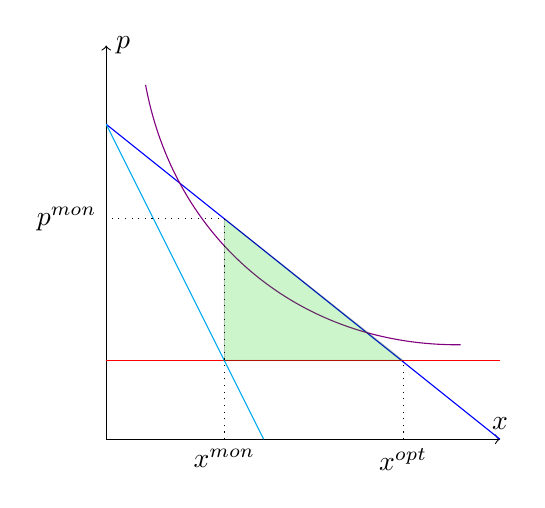
\begin{tikzpicture}
				\draw[->] (0,0) -- (5,0) node[above] {$x$};
				\draw[->] (0,0) -- (0,5) node[right] {$p$};
				
				\draw[blue] (0,4) -- (5,0);
				\draw[red] (0,1) -- (5,1);
				\draw[violet] (0.5,4.5) to[bend right=40] (4.5,1.2);
				\draw[cyan] (0,4) -- (2,0);
				
				\draw[dotted] (1.5,0) node[below] {$x^{mon}$} -- (1.5,2.8) -- (0,2.8) node[left] {$p^{mon}$};
				\draw[dotted] (3.77,0) node[below] {$x^{opt}$} -- (3.77,1);	
				\draw[fill=green!80!black,opacity=0.2] (1.5,2.8) -- (1.5,1)	-- (3.77,1) -- (1.5,2.8);
				
			\end{tikzpicture} \\
			\textcolor{blue}{GZB}, \textcolor{red}{GK}, \textcolor{cyan}{GE}, \textcolor{violet}{DK}, \textcolor{green!80!black}{Wohlfahrtsverlust}
		\end{center}
		\item Durch diese Maßnahme sinken die Kosten für den Monopolisten, sein Gewinn erhöht sich. Da die Monopolmenge aber an Grenzerlös und Grenzkosten festgemacht wird, diese sich aber nicht verschieben, ändert sich auch die Monopolmenge nicht.
		\item Der Preis wird durch diese Preisobergrenze sinken und damit wird sich auch die Menge ausdehnen, allerdings nicht auf $x^{opt}$. Der Wohlfahrtsverlust wird im Vergleich zur Situation ohne Regulierung geringer, aber er verschwindet nicht.
		\begin{center}
			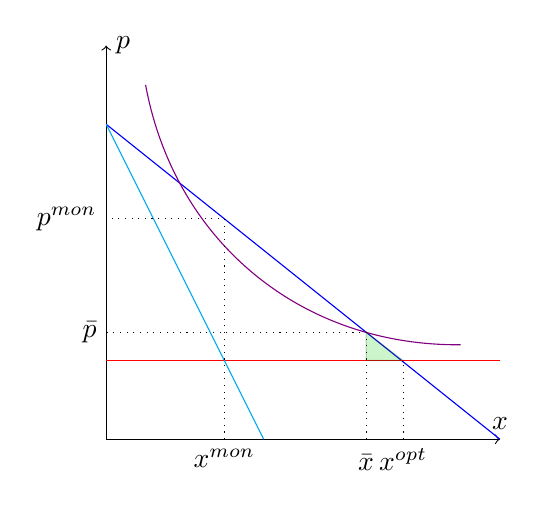
\begin{tikzpicture}
				\draw[->] (0,0) -- (5,0) node[above] {$x$};
				\draw[->] (0,0) -- (0,5) node[right] {$p$};
				
				\draw[blue] (0,4) -- (5,0);
				\draw[red] (0,1) -- (5,1);
				\draw[violet] (0.5,4.5) to[bend right=40] (4.5,1.2);
				\draw[cyan] (0,4) -- (2,0);
				
				\draw[dotted] (1.5,0) node[below] {$x^{mon}$} -- (1.5,2.8) -- (0,2.8) node[left] {$p^{mon}$};
				\draw[dotted] (3.77,0) node[below] {$x^{opt}$} -- (3.77,1);	
				\draw[dotted] (3.3,0) node[below,yshift=-2.1] {$\bar{x}$} -- (3.3,1.36) -- (0,1.36) node[left] {$\bar{p}$};
				\draw[fill=green!80!black,opacity=0.2] (3.3,1) -- (3.77,1) -- (3.3,1.36) -- (3.3,1);
				
			\end{tikzpicture} \\
			\textcolor{blue}{GZB}, \textcolor{red}{GK}, \textcolor{cyan}{GE}, \textcolor{violet}{DK}, \textcolor{green!80!black}{Wohlfahrtsverlust}
		\end{center}
	\end{enumerate}

	\section*{Aufgabe 5}
	\begin{enumerate}[label=(\alph*)]
		\item Ein natürliches Monopol zeichnet sich durch fallende Durchschnittskosten aus:
		\begin{align}
			DK &= \frac{K(x)}{x} = 75-1.5x \notag \\
			\frac{\partial DK}{\partial x} &= -1.5 \Rightarrow\text{fallend} \notag
		\end{align}
		\item Der Monopolist setzt wieder $GK=GE=E'=[120x-6x^2]'=120-12x$:
		\begin{align}
			GK &= GE \notag \\
			75-3x &= 120-12x \notag \\
			x^{mon} &= 5 \Rightarrow p^{mon}=90 \notag
		\end{align}
		\item Die optimale Menge wäre:
		\begin{align}
			GK &= GZB \notag \\
			75-3x &= 102-6x \notag \\
			x^{opt} &= 15 \notag
		\end{align}
		Bei dieser Menge macht der Monopolist eine Gewinn von
		\begin{align}
			\Pi(15) &= 15\cdot GK(15) - K(15) \notag \\
			&= 15(75-3\cdot 15) - 75\cdot 15 - 1.5\cdot 15^2 \notag \\
			&= -1012.5 \notag
		\end{align}
		Diesen Verlust muss der Staat subventionieren.
		\item Jetzt setzt der Monopolist $DK=GZB$:
		\begin{align}
			DK &= GZB \notag \\
			75-1.5x &= 120-6x \notag \\
			\bar{x} &= 10 \Rightarrow \bar{p}=60 \notag
		\end{align}
	\end{enumerate}

	\section*{Aufgabe 5}
	\begin{enumerate}[label=(\alph*)]
		\item Der Gewinn für Firma F ist $\Pi_F=x(b-dx) - (c+a)x$:
		\begin{align}
			\frac{\partial \Pi_F}{\partial x} &= b-2dx - (c+a) = 0 \notag \\
			x &= \frac{b-c-a}{2d} \Rightarrow p = b-\frac{b-c-a}{2}=\frac{a+b+c}{2} \notag
		\end{align}
		\item Der Gewinn für Firma $S$ ist $\Pi_S=xa = a\left(\frac{b-c-a}{2d}\right)$:
		\begin{align}
			\frac{\partial \Pi_S}{\partial a} &= \frac{b-c-2a}{2d} = 0 \notag \\
			0 &= b-c-2a \notag \\
			a &= \frac{b-c}{2} \notag
		\end{align}
		\item Preis = Grenzkosten = $c$
	\end{enumerate}
	
	\section*{Aufgabe 6}
	\begin{enumerate}[label=(\alph*)]
		\item Betrachten wir zuerst den Gewinn von Volta, wenn $z$ bereits festgelegt wurde:
		\begin{align}
			\Pi_V &= (46-2x)x - (c+z)x \notag \\
			&= 46x - 2x^2 - (c+z)x \notag
		\end{align}
		Dieser soll maximiert werden:
		\begin{align}
			\frac{\partial\Pi_V}{\partial x} = 46-4x - (c+z) &= 0 \notag \\
			4x &= 46 - (c+z) \notag \\
			x &= \frac{46}{4} - \frac{c+z}{4} \notag
		\end{align}
		Mit $c=2$ ergibt sich
		\begin{align}
			x = \frac{46}{4} - \frac{2+z}{4} \notag
		\end{align}
		Wenn nun Photo Corp dies antizipiert, kann Photo Corp seinen Gewinn steigern. Dazu muss es sein $z$ in Abhängigkeit von $x$ bestimmen:
		\begin{align}
			x &= \frac{46}{4} - \frac{2+z}{4} \notag \\
			\frac{2+z}{4} &= \frac{46}{4} - x \notag \\
			2+z &= 46-4x \notag \\
			z &= 44-4x \notag
		\end{align}
		Der Gewinn ergibt sich nun
		\begin{align}
			\Pi_P &= z\cdot x - (10+4x) \notag \\
			&= (44-4x)x - (10+4x) \notag \\
			&= 44x-4x^2-10-4x \notag \\
			&= 40x - 4x^2 - 10 \notag
		\end{align}
		Dieser soll nun maximiert werden:
		\begin{align}
			\frac{\partial\Pi_P}{\partial x} = 40-8x &= 0 \notag \\
			40 &= 8x \notag \\
			x &= 5 \notag
		\end{align}
		Mit $x=5$ ergibt sich $z = 44-4\cdot 5 = 24$ und $p=46-2\cdot 5 = 36$.
		\item Der Gewinn des neuen Monopols ist
		\begin{align}
			\Pi &= (46-2x)x - (10+4x) - 2x \notag \\
			&= 46x-2x^2-10-4x - 2x \notag \\
			&= 40x-2x^2-10 \notag
		\end{align}
		Auch dieser soll maximiert werden:
		\begin{align}
			\frac{\partial\Pi}{\partial x} = 40-4x&=0 \notag \\
			40 &= 4x \notag \\
			x &= 10 \notag
		\end{align}
		Damit ergibt sich ein Preis von $p=46-2\cdot 10= 26$.
		\item Photo Corp sollte seine Gewinne im Fall des Doppelmonopols $\Pi_{Doppelm.}$ und im Fall der Übernahme ($\Pi_{Kauf}$) berechnen. Die Differenz dazwischen sind die maximalen Kosten, die Photo Corp bereit wäre zu bezahlen.
		\begin{align}
			\Pi_{Doppelm.} &= zx - K(x) \notag \\
			&= 24\cdot 5 - (10+4\cdot 5) \notag \\
			&= 90 \notag \\
			\Pi_{Kauf} &= px - K(x) - cx \notag \\
			&= 26\cdot 10 - (10+4\cdot 10) - 2\cdot 10 \notag \\
			&= 190 \notag
		\end{align}
		Photo Corp sollte Volta nur dann übernehmen, wenn die Kosten $S$ kleiner als $190-90=100$ sind.
		\item Die gesamtwirtschaftlich optimale Länge, ist dann erreicht, wenn $GK=GZB$ ist. Es gilt $GK = c + \frac{\partial K}{\partial x} = c + 4$. Also
		\begin{align}
			2+4 &= 46-2x \notag \\
			2x &= 40 \notag \\
			x &= 20 \notag
		\end{align}
		Damit ergibt sich $p=46-2\cdot 20=6$.
		\item Gesamtwirtschaftlich am besten ist es, wenn es vollständige Konkurrenz gibt, also möglichst wenig Marktmacht. Das heißt auch, dass ein Monopol besser ist als 2 hintereinandergeschaltete Monopole. Die Marktmacht kann mittels Zerschlagung von Monopolen, Subvention der Monopole oder Preisgrenzen begrenzt werden.
	\end{enumerate}

	\section*{Zusatzaufgabe 2}
	\begin{enumerate}[label=(\alph*)]
		\item Der Gewinn von FONA ist $\Pi_F=D(p_T)\cdot a_F - D(p_T)\cdot c$:
		\begin{align}
			\frac{\partial \Pi_F}{\partial a_F} &= -a_F\left(1-\frac{1}{\eta}\right)^\eta\eta(a_F+c)^{-\eta-1} + c\left(1-\frac{1}{\eta}\right)^\eta\eta(a_F+c)^{-\eta-1} = 0 \notag \\
			0 &= \left(\frac{\eta-1}{\eta}\right)^\eta(a_F+c)^{-\eta-1}(-a_F\eta+a_F+c\eta+c) \notag \\
			a_F &= \frac{c(\eta+1)}{\eta-1} \Rightarrow p_T = \frac{\eta(c(\eta-1)+c(\eta+1))}{(\eta-1)^2} \notag
		\end{align}
		\item Nur die Grenzkosten $a_F=c$. Die Gesellschaft maximiert ihren Gewinn $\Pi_G=p\cdot D(p) - 2cD(p)$:
		\begin{align}
			\frac{\partial\Pi_G}{\partial p} &= 2c\eta p^{-\eta-1} - \eta p^{-\eta} + p^{-\eta} = 0 \notag \\
			p &= \frac{2c\eta}{\eta-1} \notag
		\end{align}
		\item In der Optimallösung sollte $a_F=c$ und $p=2c$ sein.
		\item Gesamtwirtschaftlich am besten ist es, wenn es vollständige Konkurrenz gibt, also möglichst wenig Marktmacht. Das heißt auch, dass ein Monopol besser ist als 2 hintereinandergeschaltete Monopole. Die Marktmacht kann mittels Zerschlagung von Monopolen, Subvention der Monopole oder Preisgrenzen begrenzt werden.
	\end{enumerate}

\end{document}